\documentclass[12pt]{article}

\input{../preambleProblemSets}



\hspace*{\fill}\textbf{\Large Problem set 9}\hspace*{\fill}

\hrulefill

\newcommand{\T}{^{\mathsf T}}
\newcommand{\bK}{\overline{\mathbf K}}
\newcommand{\bM}{\overline{\mathbf M}}
\newcommand{\vct}[1]{\mathbf{#1}}
\newcommand{\colv}[1]{\begin{bmatrix}#1\end{bmatrix}}



\begin{document}

\noindent ME473 - Dynamic finite element analysis of structures\hfill EPFL\\
Stefano Burzio \hfill 2025\\
\vspace{0.3cm}
\coursehead{Problem set 10}
\ptitle{Problem 1 \quad Two Ritz vectors for a free-free shaft}
Use MATLAB for this problem. In Problem Set 9, a single linear element gave
$\omega_1=\sqrt{12G/\rho}/\ell$ for the first elastic torsional mode. Keep the
uniform shaft of length $\ell$, shear modulus $G$, density $\rho$ and polar
moment $I_p$. Both ends are torque-free. Use four equal linear elements of
length $h=\ell/4$ and retain all five nodal rotations.
\begin{center}
  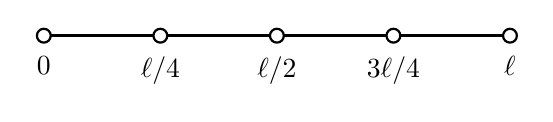
\begin{tikzpicture}[x=1.48cm,y=1cm]
    \draw[line width=1pt] (0,0)--(4,0);
    \foreach \j/\lab in {0/0,1/{\ell/4},2/{\ell/2},3/{3\ell/4},4/{\ell}} {
    \filldraw[fill=white,draw=black,thick] (\j,0) circle (2.5pt);
    \node[below=4pt] at (\j,0) {$\lab$};
    }
  \end{tikzpicture}
\end{center}
Use $\lambda=\omega^2$ and report the dimensionless quantities
\[
  \bK=\frac{\ell}{GI_p}\vct K,\quad
  \bM=\frac{\vct M}{\rho I_p\ell},\quad
  \Lambda=\frac{\rho\ell^2}{G}\lambda,\qquad
  \Omega=\sqrt{\Lambda}.
\]
Number the modes from $k=0$ (rigid rotation). The target pair is $k=0,1$.
\begin{enumerate}
  \item \textbf{Assemble and solve the full model.}
        Assemble $\bK$ and $\bM$ using the element stiffness and consistent mass
        matrices from Problem Set 9. Solve $\bK\vct p=\Lambda\bM\vct p$ with
        \texttt{eig}, sort the five eigenpairs, and check $\bK\vct 1=\vct 0$.
        Compare the frequencies and nodal shapes with the exact continuum modes
        $\Omega_k=k\pi$, $\varphi_k(x)=\cos(k\pi x/\ell)$, for $k=0,\ldots,4$.
  \item \textbf{Reduce from five coordinates to two.}
        Use the two columns of $\vct\Psi_g$ below. The second column samples the
        smooth twist $16(1-6s^2+4s^3)$ at $s=x/\ell$.
        Form $\vct K^*=\vct\Psi\T\bK\vct\Psi$ and
        $\vct M^*=\vct\Psi\T\bM\vct\Psi$, solve the $2\times2$ pencil and recover
        both five-component modes as $\widehat{\vct p}=\vct\Psi\vct y$.
        \[
          \vct\Psi_g=\colv{1&16\\1&11\\1&0\\1&-11\\1&-16},
          \qquad
          \vct\Psi_b=\colv{2&0\\-1&1\\0&-2\\-1&1\\2&0}.
        \]
  \item \textbf{Measure the accuracy.} Compare both Ritz pairs with the full
        FE reference. Use the absolute error for $\Lambda_0=0$, a percentage error
        for $\Lambda_1$, and the following scale- and sign-independent shape measure:
        \[
          \operatorname{MAC}_{\bM}(\vct u,\vct v)=
          \frac{|\vct u\T\bM\vct v|^2}{(\vct u\T\bM\vct u)(\vct v\T\bM\vct v)}.
        \]
        For the first elastic mode also compare $\widehat\Omega_1$ with $\pi$ and
        with the one-element result. Plot the exact and approximate shapes together.
  \item \textbf{Try a different space.} Repeat the reduction and error checks
        with $\vct\Psi_b$. Identify which full FE modes are returned. Use reflection
        about the midpoint and $\vct 1\T\bM\vct\Psi_b$ to explain what happens.
\end{enumerate}
\newpage
\ptitle{Problem 2 \quad Two steps of inverse Lanczos by hand}
Use pen and paper. Return to Problem 2 of Problem Set 9. A single quadratic
element models the axial vibration of a uniform free-free bar, with its
degrees of freedom ordered \emph{left end, midpoint, right end}. With
$c=E/(\rho\ell^2)$, its stiffness and lumped mass matrices are
\[
  \vct K=\frac{EA}{3\ell}\vct C,\qquad
  \vct M=\frac{\rho A\ell}{6}\vct D,\qquad
  \vct C=\colv{7&-8&1\\-8&16&-8\\1&-8&7},\quad
  \vct D=\operatorname{diag}(1,4,1).
\]
Retain the shift $\sigma=2c$. Write $\mu=\lambda/c$ and
$\mu_\sigma=(\lambda+\sigma)/c=\mu+2$. To keep the hand calculation short,
the scaled inverse operator is supplied:
\[
  \vct B=14c(\vct K+2c\vct M)^{-1}\vct M
  =\frac1{13}\colv{24&56&11\\14&63&14\\11&56&24},
  \qquad \langle\vct u,\vct v\rangle_D=\vct u\T\vct D\vct v .
\]
\begin{enumerate}
  \item \textbf{Set up the recurrence.} Show that $\vct D\vct B$ is symmetric.
        If $\vct B\vct p=\nu\vct p$, derive $\mu_\sigma$ and $\mu$ from $\nu$.
        Normalize $\vct g=(2,1,0)\T$ in the $D$-norm to obtain $\vct q_1$.
  \item \textbf{Take two Lanczos steps.} Start with $\vct q_0=\vct0$ and
        $\beta_0=0$. For $j=1,2$, use
        \[
          \alpha_j=\langle\vct q_j,\vct B\vct q_j\rangle_D,\qquad
          \vct w_j=\vct B\vct q_j-\alpha_j\vct q_j-\beta_{j-1}\vct q_{j-1},
          \qquad \beta_j=\|\vct w_j\|_D .
        \]
        Set $\vct q_{j+1}=\vct w_j/\beta_j$ when $\beta_j>0$.
        Compute $\alpha_1,\beta_1,\vct q_2,\alpha_2,\beta_2$ and assemble $\vct T_2$.
        What estimate of the lowest $\mu$ was already available after step 1?
  \item \textbf{Recover and identify the two modes.} Solve the $2\times2$
        problem $\vct T_2\vct y=\nu\vct y$. For each root, recover $\mu$ and
        $\widehat{\vct p}=[\vct q_1,\vct q_2]\vct y$. Scale each shape to have
        left-end value $1$. Verify each pair directly in $2\vct C\vct p=\mu\vct D\vct p$.
  \item \textbf{Compare with subspace iteration.} The table gives the results
        of the three block inverse iterations specified in Problem Set 9, from
        $\vct P_{(0)}\propto[\vct e_1,\vct e_2]$. Use it directly.
        Compare shifted eigenvalues and mode shapes with your Lanczos results and
        the exact pairs. For each method, give the relative error in $\mu_\sigma$
        and identify the largest nodal discrepancy at the common left-end scaling.
        Explain why Lanczos terminates after two steps for this start.
\end{enumerate}
\begin{center}
  \begin{tabular}{@{}cll@{}}
    \toprule
    Mode          & $\mu_\sigma$ after three iterations & Mode shape, left end $=1$                           \\
    \midrule
    Rigid         & $2.000002317$                       & $(1,\ \phantom{-}1.000438,\ \phantom{-}0.999603)\T$ \\
    First elastic & $14.423259$                         & $(1,\ -0.067550,\ -0.729971)\T$                     \\
    \bottomrule
  \end{tabular}
\end{center}
\newpage
\ptitle{Problem 3 \quad Choosing a Jacobi pivot}
Work by hand. Let $\vct K=\vct K\T$ and $\vct M=\vct M\T\succ0$. Pick
$i<j$ and use the current principal blocks
\[
  \vct K_p=\colv{k_{ii}&k_{ij}\\k_{ij}&k_{jj}},\qquad
  \vct M_p=\colv{m_{ii}&m_{ij}\\m_{ij}&m_{jj}} .
\]
Each transformation acts only on coordinates $i,j$. Use the congruence
convention $\vct K_p'=\vct J\T\vct K_p\vct J$ and
$\vct M_p'=\vct J\T\vct M_p\vct J$.
\begin{enumerate}
  \item \textbf{One pivot in the standard problem.} Take $\vct M_p=\vct I$ and
        \[
          \vct J=\vct R(\theta)=
          \colv{\cos\theta&-\sin\theta\\ \sin\theta&\cos\theta}.
        \]
        Multiply the two pivot columns against $\vct K_p$ to obtain the
        off-diagonal entry of $\vct K_p'$. Set it to zero and verify that
        \[
          \tan(2\theta)=\frac{2k_{ij}}{k_{ii}-k_{jj}},\qquad |\theta|\leq\pi/4 .
        \]
        Explain the choice of angle when $k_{ij}=0$ or $k_{ii}=k_{jj}$.
  \item \textbf{One pivot pair in the generalized problem.} Use
        $\vct J=\bigl[\begin{smallmatrix}1&\alpha\\\gamma&1\end{smallmatrix}\bigr]$.
        Show that simultaneous elimination of the stiffness and mass off-diagonal
        entries requires
        \begin{align*}
          k_{ii}\alpha+k_{jj}\gamma+k_{ij}(1+\alpha\gamma) & =0, \\
          m_{ii}\alpha+m_{jj}\gamma+m_{ij}(1+\alpha\gamma) & =0.
        \end{align*}
  \item \textbf{Find $\alpha$ and $\gamma$.} Introduce the quantities used in
        the lecture,
        \[
          \bar k_{ii}=k_{ii}m_{ij}-m_{ii}k_{ij},\quad
          \bar k_{jj}=k_{jj}m_{ij}-m_{jj}k_{ij},\quad
          \bar k=\tfrac12(k_{ii}m_{jj}-k_{jj}m_{ii}).
        \]
        Eliminate $1+\alpha\gamma$ to find a relation between the two unknowns.
        Write $\alpha=\bar k_{jj}/x$, $\gamma=-\bar k_{ii}/x$ and derive the
        quadratic satisfied by $x$. Which root has the larger magnitude, and why
        is it preferable when evaluating the formula? For $\vct M_p=\vct I$,
        show how normalizing the columns recovers $\vct R(\theta)$.
  \item \textbf{Check a numerical pivot.} Use
        \[
          \vct K_p=\colv{3&1\\1&7},\qquad \vct M_p=\colv{1&1\\1&4}.
        \]
        First apply the standard angle chosen from $\vct K_p$ and check the mass
        off-diagonal entry. Then compute $x,\alpha,\gamma$ using part (c).
        Multiply out both generalized congruences and read the two generalized
        eigenvalues from the diagonal entries.
\end{enumerate}
\end{document}
